\documentclass[10pt,letterpaper]{article}

\usepackage[letterpaper,margin=0.70in,headheight=22pt,headsep=16pt,footskip=24pt]{geometry}
\usepackage[T1]{fontenc}
\usepackage[utf8]{inputenc}
\usepackage{lmodern}
\usepackage{microtype}
\usepackage{xcolor}
\usepackage{graphicx}
\usepackage{booktabs}
\usepackage{array}
\usepackage{tabularx}
\usepackage{longtable}
\usepackage{amsmath,amssymb}
\usepackage{tikz}
\usetikzlibrary{arrows.meta,positioning,calc,shapes.geometric,decorations.pathreplacing,fit}
\usepackage{enumitem}
\usepackage{fancyhdr}
\usepackage{titlesec}
\usepackage{caption}
\usepackage{listings}
\usepackage{xurl}
\usepackage[hidelinks]{hyperref}
\usepackage{lastpage}
\usepackage{float}
\usepackage{placeins}
\usepackage{needspace}

% WVURAIL house palette: shared neutrals, per-project accent.
% PilotProxy uses FStatRed (A00000); datatrawl uses TrawlAmber.
\definecolor{TrawlAmber}{HTML}{A66A00}
\definecolor{TrawlGray}{HTML}{555555}
\definecolor{TrawlBlue}{HTML}{144E8C}
\definecolor{LightGray}{HTML}{F3F3F3}
\definecolor{MidGray}{HTML}{D9D9D9}
\definecolor{DarkText}{HTML}{1A1A1A}
\definecolor{GoodGreen}{HTML}{2B7A2B}
\definecolor{WarnOrange}{HTML}{A65E00}

\renewcommand{\familydefault}{\sfdefault}
\setlength{\parindent}{0pt}
\setlength{\parskip}{5pt}
\renewcommand{\arraystretch}{1.15}
\sloppy
\setlist[itemize]{leftmargin=1.2em,itemsep=2pt,topsep=2pt}
\setlist[enumerate]{leftmargin=1.4em,itemsep=2pt,topsep=2pt}

\titleformat{\section}{\Large\bfseries\color{DarkText}}{}{0pt}{}[\vspace{-3pt}\color{TrawlAmber}\titlerule]
\titleformat{\subsection}{\large\bfseries\color{DarkText}}{}{0pt}{}
\titleformat{\subsubsection}{\normalsize\bfseries\color{DarkText}}{}{0pt}{}

\newcommand{\code}[1]{\texttt{\detokenize{#1}}}
\newcommand{\apicode}[1]{\texttt{\detokenize{#1}}}
\newcommand{\yes}{\textcolor{GoodGreen}{Yes}}
\newcommand{\no}{\textcolor{TrawlGray}{No}}
\newcolumntype{Y}{>{\raggedright\arraybackslash}X}
\newcolumntype{L}[1]{>{\raggedright\arraybackslash}p{#1}}
\newcolumntype{C}[1]{>{\centering\arraybackslash}p{#1}}
\captionsetup{font=small,labelfont=bf}

\lstdefinestyle{shell}{
  basicstyle=\ttfamily\footnotesize,
  breaklines=true,
  columns=fullflexible,
  frame=single,
  rulecolor=\color{MidGray},
  backgroundcolor=\color{LightGray},
  keepspaces=true,
  showstringspaces=false
}
\lstset{style=shell}

\newcommand{\notebox}[1]{%
  \vspace{4pt}\noindent\fcolorbox{TrawlBlue}{LightGray}{%
  \begin{minipage}{0.965\linewidth}%
  \textbf{Note:} #1%
  \end{minipage}}\vspace{4pt}}

\newcommand{\importantbox}[1]{%
  \vspace{4pt}\noindent\fcolorbox{TrawlAmber}{LightGray}{%
  \begin{minipage}{0.965\linewidth}%
  \textbf{Important:} #1%
  \end{minipage}}\vspace{4pt}}

\newcommand{\field}[1]{\texttt{\detokenize{#1}}}

\pagestyle{fancy}
\fancyhf{}
\fancyhead[L]{\small Datatrawl-DS001}
\fancyhead[C]{\small Storage-Safe Archive Trawling Engine v1.0.0}
\fancyhead[R]{\small Product Specification}
\fancyfoot[L]{\small Datatrawl-DS001 v1.3}
\fancyfoot[C]{\small West Virginia University}
\fancyfoot[R]{\small Page \thepage\ of \pageref{LastPage}}
\renewcommand{\headrulewidth}{0.8pt}
\renewcommand{\headrule}{\hbox to\headwidth{\color{TrawlAmber}\leaders\hrule height \headrulewidth\hfill}}
\renewcommand{\footrulewidth}{0.8pt}
\renewcommand{\footrule}{\hbox to\headwidth{\color{TrawlAmber}\leaders\hrule height \footrulewidth\hfill}}

\title{datatrawl Storage-Safe Archive Trawling Engine v1.0.0\\Product Specification}
\author{West Virginia University}
\date{Datatrawl-DS001 v1.3 \\ July 10, 2026}
\hypersetup{
  pdftitle={datatrawl Storage-Safe Archive Trawling Engine v1.0.0 -- Product Specification},
  pdfauthor={West Virginia University Radio Astronomy Instrumentation Lab (RAIL)},
  pdfsubject={Datatrawl-DS001 v1.3},
  pdfkeywords={datatrawl, radio astronomy, archive analysis, resumable processing}
}

\begin{document}
\thispagestyle{fancy}
{\sffamily
\begin{minipage}[t]{0.39\textwidth}
  {\fontsize{24}{26}\selectfont\bfseries\color{TrawlAmber}datatrawl}\par
  {\small Datatrawl-DS001 v1.3, July 10, 2026}
\end{minipage}%
\begin{minipage}[t]{0.61\textwidth}
  \raggedleft
  {\large\bfseries Storage-Safe Archive Trawling Engine}\par
  {\small Bounded staging. Resumable. Provenance-carrying.}\par
  {\small West Virginia University Radio Astronomy Instrumentation Lab (RAIL)}
\end{minipage}
}
\vspace{6pt}
{\color{TrawlAmber}\hrule height 1.2pt}
\vspace{8pt}

{\small\color{TrawlGray}Long archive analyses must operate within scratch-space
limits and must continue after interrupted sessions. This specification defines
the datatrawl v1.0.0 engine contract for that problem. Datatrail/CADC remains
the source of record for archive contents. datatrawl builds an
analysis-specific inventory, processes staged copies under an explicit
file-count bound, checkpoints the result, and removes each copy after use.
Throughput depends on the source, network, file size, and analyzer, and must be
measured on the target system.}

\section{Features}
\begin{itemize}
  \item \textbf{Bounded staging}: the default run stages and analyzes one file
        at a time. \code{--max-staged-files} permits bounded prefetching, and
        the engine removes each staged copy after it is consumed.
  \item \textbf{Resumable products}: the analyzer owns the product and records
        the units committed at each checkpoint. A repeated command skips those
        recorded units. Work completed after the last checkpoint may be
        repeated after an interruption.
  \item \textbf{Four-part run model}: a run selects a \field{telescope},
        \field{source}, \field{reader}, and \field{analyzer}.
        \code{datatrawl doctor} checks the selected combination before a long
        scan is started.
  \item \textbf{External plugins}: sources, readers, and analyzers register
        through the \code{datatrawl.plugins} entry-point group or an explicit
        \code{--plugin} module path. A project can therefore supply its own
        analysis without modifying datatrawl.
  \item \textbf{Ordering contract}: an order-dependent analyzer sets
        \field{requires_in_order}. The engine then rejects settings that may
        deliver files in download-completion order.
  \item \textbf{Persistent inventories}: \code{datatrawl survey} records the
        telescope, source, and reader in a named inventory directory. A later
        \code{datatrawl scan} needs the inventory and analyzer. The current
        engine loads the units selected for one product into memory before
        staging begins.
  \item \textbf{Selection}: \field{freq_id}s and/or events, one grammar
        across sources --- \code{614,706}, \code{506-844},
        \code{events:349382977}, or the dict form a \field{plan_runs}
        returns; filters are exact and ANDed, and malformed input fails
        loudly with the grammar named.
  \item \textbf{Archive discovery}: \code{survey --scopes-only}
        maps scopes and datasets without enumerating events or downloading data;
        \code{--match} filters by name, \code{--expand} opens containers one
        level, and \code{--name} labels the map. If Datatrail does not answer
        for a scope, datatrawl marks the map INCOMPLETE instead of treating the
        missing response as an empty scope.
  \item \textbf{Reader-owned archive file shape}: which files one event
        contributes is declared by the reader (\field{survey_files});
        each inventory row records its file \field{name}. A later scan uses
        that recorded name rather than reconstructing the current naming rule.
  \item The supplied analyzer base class and spectrum analyzer checkpoint
        through a temporary file followed by \field{os.replace}; automatically
        created staging directories are unique to one invocation; and the
        analyzer owns unit-key provenance.
  \item Pure-Python core (\code{numpy}, \code{h5py}, \code{pyyaml});
        CANFAR/CADC access and GPU acceleration are optional extras.
\end{itemize}

\clearpage
\section{What datatrawl Is and Is Not}
\begin{tabularx}{\linewidth}{L{0.30\linewidth} Y}
\toprule
\textbf{Is} & A run layer that walks an archive inventory, analyzes one staged
              file at a time, hands its arrays to a science analyzer, saves a
              resumable product, and deletes the staged copy after use. The
              engine may overlap that serial consumption with an explicitly
              bounded fetch queue. \\
\textbf{Is} & A contract between an engine and plugins. The contract defines
              lifecycle, ordering, resume, and provenance behavior for long
              unattended runs. \\
\textbf{Is not} & An archive. Datatrail/CADC remain the authority on what data
              exists and where; datatrawl never mutates archive state. \\
\textbf{Is not} & A scheduler or workflow manager. One \code{scan} is one
              process; independence across products comes from the analyzer's
              \field{plan_runs} split, not from a DAG engine. \\
\textbf{Is not} & A science package. The statistics live in analyzers
              (built-in \code{spectrum}, or external plugins such as the
              PilotProxy detector). \\
\bottomrule
\end{tabularx}

\section{System Overview}
\begin{figure}[H]
\centering
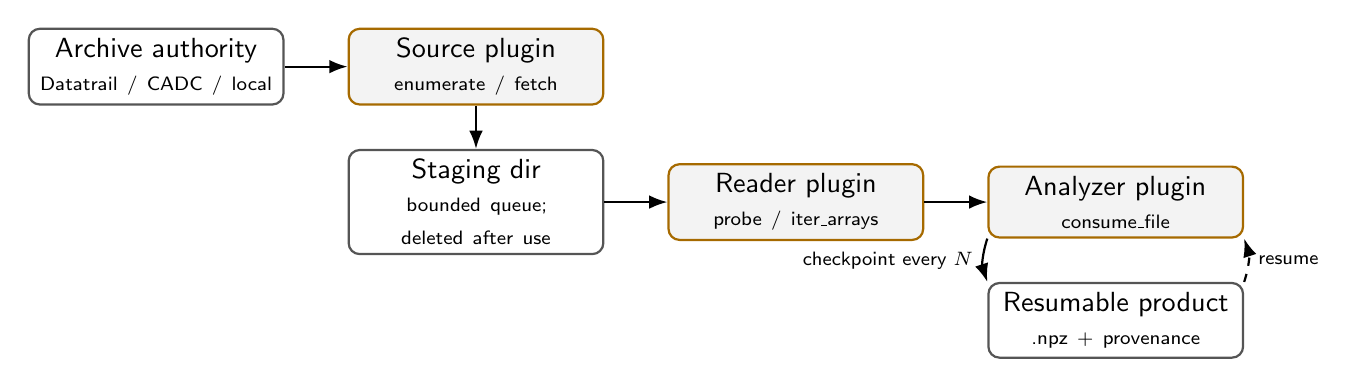
\begin{tikzpicture}[node distance=0.55cm and 0.8cm,>=Latex]
\tikzstyle{blk}=[rectangle,rounded corners,draw=TrawlAmber,thick,fill=LightGray,
                 minimum height=0.85cm,text width=3.0cm,align=center]
\tikzstyle{soft}=[rectangle,rounded corners,draw=TrawlGray,thick,fill=white,
                  minimum height=0.85cm,text width=3.0cm,align=center]
\node[soft] (arch) {Archive authority\\{\scriptsize Datatrail / CADC / local}};
\node[blk,right=of arch] (src) {Source plugin\\{\scriptsize enumerate / fetch}};
\node[soft,below=of src] (stage)
  {Staging dir\\{\scriptsize bounded queue; deleted after use}};
\node[blk,right=of stage] (rdr)
  {Reader plugin\\{\scriptsize probe / iter\_arrays}};
\node[blk,right=of rdr] (ana) {Analyzer plugin\\{\scriptsize consume\_file}};
\node[soft,below=of ana] (prod) {Resumable product\\{\scriptsize .npz + provenance}};
\draw[->,thick] (arch) -- (src);
\draw[->,thick] (src) -- (stage);
\draw[->,thick] (stage) -- (rdr);
\draw[->,thick] (rdr) -- (ana);
\draw[->,thick]
  (ana.south west) to[bend right=18]
  node[left,font=\scriptsize]{checkpoint every $N$} (prod.north west);
\draw[->,thick,dashed]
  (prod.north east) to[bend right=18]
  node[right,font=\scriptsize]{resume} (ana.south east);
\end{tikzpicture}
\caption{datatrawl processing sequence. The source stages one unit, the reader
streams arrays from that unit, and the analyzer updates its product. The engine
removes the staged copy and asks the analyzer to checkpoint at the configured
interval.}
\end{figure}

\clearpage
\section{Operating Limits and Contracts}
\begin{tabularx}{\linewidth}{L{0.34\linewidth} L{0.22\linewidth} Y}
\toprule
\textbf{Parameter} & \textbf{Value} & \textbf{Contract} \\
\midrule
Staged files on disk & 1 (default) & \code{--max-staged-files} raises the
prefetch depth; refused when the analyzer sets \field{requires_in_order}. \\
Staged-input footprint & Approximately $N S_{\max}$ & $N$ is
\code{--max-staged-files} and $S_{\max}$ is the largest selected file;
product-checkpoint temporary space and filesystem overhead are additional. \\
Download workers & 1 (default) & Adds fetch threads; concurrent fetches also
require more than one staging slot. Accumulator writes stay on the engine's
main thread (no analyzer locking). Refused for in-order analyzers. \\
Checkpoint interval & 50 consumed files & \code{--checkpoint-every}; the
engine calls the analyzer's \code{save()} for the full product after this many
successful units. \\
Delivery order & Source order & Guaranteed when
\code{--download-workers=1} and \code{--max-staged-files=1}. With relaxed
settings, delivery order is not part of the public contract and may follow
fetch completion. \\
Staging directory & Unique when automatic & Without \code{--tmp-dir}, each
scan receives a unique directory under \code{DATATRAWL_TMPDIR}, writable
\code{/scratch}, or the operating-system temporary directory. An explicit
\code{--tmp-dir} is used as-is and must not be shared by concurrent scans. \\
Supplied product write & Atomic replacement & The base class and spectrum
analyzer write a temporary file in the product directory and then call
\field{os.replace}. An external analyzer owns the equivalent obligation. \\
Resume gate & Analyzer-defined & \field{resume()} must reject an existing
product when a changed parameter would alter its meaning. \\
Inventory memory & Selection-sized & Inventory rows persist on disk between
commands, but \code{scan} materializes the units selected for each product in
memory before processing. Memory use grows with the selected inventory. \\
\bottomrule
\end{tabularx}

\Needspace{0.32\textheight}
\section{Command Surface}
\begin{tabularx}{\linewidth}{L{0.28\linewidth} Y}
\toprule
\textbf{Command} & \textbf{Function} \\
\midrule
\code{datatrawl list} & List the registered components; subcommands
\code{telescopes}, \code{readers}, \code{analyzers}, \code{sources}. \\
\code{datatrawl doctor} & Report usable combinations; with
\code{--telescope/--source/--reader/--analyzer}, the checklist for one chosen
combination. \\
\code{datatrawl explore} & Summarize an existing archive inventory or a local
directory (no staging or bulk download). \\
\code{datatrawl survey} & Walk the archive to build a named inventory
directory; records telescope, source, and reader. With \code{--scopes-only},
recon: map scopes and datasets (\code{--match}, \code{--expand},
\code{--name}) with no event enumeration or download. \\
\code{datatrawl scan} & Run the streaming analyzer over an inventory
(\code{--name}/\code{--inventory}), with \code{--select} interpreted by the
analyzer. \\
\code{datatrawl setup-cupy} & Detect the session image's CUDA version and
report the matching \code{cupy-cudaXXx} wheel; add \code{--install} to install
that wheel into the active environment. \\
\code{datatrawl --version} & Package and runtime report the same version. \\
\bottomrule
\end{tabularx}

\section{Plugin Interfaces}
\subsection{Analyzer lifecycle}
The analyzer owns the product file. It writes the product, reloads it on
resume, and reports the units already committed. The engine calls:
\begin{lstlisting}
resume(path, ctx) -> bool     # load an existing, compatible product
processed_keys()  -> set      # Unit.key values already accumulated
begin(ctx, first_meta)        # once, at the first new file
consume_file(arrays, meta)->n # per file; update accumulators
save(path)                    # persist a resumable product + provenance
summary()         -> dict     # one human-readable status line
\end{lstlisting}
Selection hooks \field{resolve_selection} and \field{plan_runs} let an
analyzer interpret \code{--select} and split it into independent, individually
resumable products (e.g.\ one product per \field{freq_id}).

\importantbox{Set \field{requires_in_order = True} when the product depends on
consume order, including running statistics, CFAR baselines, and trailing
windows. The engine then rejects \code{--download-workers}\,/\,%
\code{--max-staged-files} above 1.}

\subsection{Source and Reader}
\begin{itemize}
  \item \textbf{Source}: \field{enumerate(ctx)} yields \field{Unit}s;
        \field{fetch(unit, dest)} stages one file; \field{survey(ctx, out)}
        builds an inventory; \field{preflight(ctx)} lets \code{datatrawl
        doctor} verify credentials and connectivity before the user starts a
        run.
  \item \textbf{Reader}: \field{probe(path)} returns file metadata;
        \field{iter_arrays(path, ctx)} streams decode-ready arrays;
        \field{preflight(ctx)} lets \code{datatrawl doctor} verify decode
        prerequisites. Optionally,
        \field{survey_files(event, common_path, selection, ctx)} declares the
        archive file shape for surveys, and \field{annotate_row} enriches
        verified inventory rows.
\end{itemize}
The Datatrail adapter, re-exported from \code{datatrawl.plugins.sources}, is
the one sanctioned dtcli surface for analyzers and user code;
\field{DATATRAIL.files(scope, dataset)} lists a dataset's files
programmatically (the \code{datatrail ps -s} view) with a contract that
distinguishes a service outage from an empty dataset.

\subsection{Registration}
Plugins register through the \code{datatrawl.plugins} entry-point group, or
explicitly at run time with \code{--plugin yourpkg.module}. The PilotProxy
package registers its \code{chime-baseband-packed} reader and its detector
analyzers this way.

\section{Provenance and Resume Semantics}
Each analyzer owns its product and resume contract. It must persist every
\field{Unit.key} committed to the product and each parameter that changes the
product's meaning. \field{resume()} must reject an incompatible product. The
supplied accumulating base class provides committed-key storage and atomic NPZ
replacement. The spectrum analyzer extends it with parameter validation for its
supported fields. On restart, the engine obtains the committed keys through
\field{processed_keys()} and skips matching units. A process
interruption can therefore require the files consumed since the last completed
checkpoint to be processed again. In the supplied implementations, the previous
checkpoint remains available because replacement occurs only after the new
temporary product has been written. An external analyzer must provide equivalent
atomic-replacement behavior if it is to make the same recovery claim for an
ordinary process interruption.

\section{Environment and Dependencies}
\begin{tabularx}{\linewidth}{L{0.24\linewidth} L{0.30\linewidth} Y}
\toprule
\textbf{Extra} & \textbf{Packages} & \textbf{Enables} \\
\midrule
(core) & \code{numpy}, \code{h5py}, \code{pyyaml} & Engine, instruments,
built-in reader/analyzer. \\
\code{[cadc]} & \code{cadcdata}, \code{cadcutils} & CADC fetch path. \\
\code{[survey]} & \code{cadcdata}, \code{cadcutils},
\code{datatrail-cli>=0.11.0} & Datatrail inventory builds and CADC fetch. \\
\code{[gpu]} & (none pinned) & GPU analyzers; CuPy is installed to match the
image's CUDA via \code{datatrawl setup-cupy --install}. \\
\code{[dev]} & \code{pytest}, \code{build}, \code{twine} & Test and release
tooling. \\
\bottomrule
\end{tabularx}

Python $\geq$ 3.9. Continuous integration runs the full suite on CPython
3.9--3.14 and smoke-tests the built wheel (including
\code{datatrawl --version} and instrument loading) outside the source tree.

\section{Compliance and Testing}
\begin{itemize}
  \item The pytest suite exercises the engine loop, kill/resume, ordering
        refusal, atomic writes, inventory handling, CLI output, the built-in
        plugins, the selection grammar, recon (including outage handling),
        and the per-event/companion composition end to end through the CLI.
  \item The release job builds the source distribution and wheel, runs
        \code{twine check}, installs the wheel in a new virtual environment,
        and verifies the Datatrail dependency
        contract.
  \item License: MIT. Machine-readable citation in \code{CITATION.cff};
        release notes in \code{CHANGELOG.md}.
\end{itemize}

\section{Related Documents}
\begin{itemize}
  \item \textbf{Datatrawl-UG001} --- User Guide (install, quickstart, CANFAR
        runbook, writing plugins, troubleshooting).
  \item \code{docs/ADDING_AN_ANALYZER.md}, \code{ADDING_A_READER.md},
        \code{ADDING_A_SOURCE.md}, \code{ADDING_A_TELESCOPE.md} --- extension
        guides.
  \item \code{docs/DATATRAIL_BOUNDARY.md} --- the authority boundary between
        datatrawl and the Datatrail archive.
  \item \textbf{PilotProxy-DS001/UG001} --- the RAIL detector package built on
        this engine.
\end{itemize}

\Needspace{0.24\textheight}
\section{Revision History}
\begin{tabularx}{\linewidth}{L{0.12\linewidth} L{0.20\linewidth} Y}
\toprule
\textbf{Rev} & \textbf{Date} & \textbf{Changes} \\
\midrule
v1.0 & July 1, 2026 & Initial release, documenting engine v0.1.0. \\
v1.1 & July 3, 2026 & Engine v0.2.0: recon (\code{--scopes-only} with
\code{--match}/\code{--expand}/\code{--name}, telescope-scoped), event
selection grammar, reader-owned archive file shape (\code{survey --reader}),
\code{DATATRAIL.files()}, per-event fan-out and companion patterns. \\
v1.2 & July 3, 2026 & Version designation: engine v0.2.0 redesignated v1.0.0
under the 1.0 stability contract (public CLI, plugin contracts,
product/inventory formats); no functional changes. External analyzer example
moved to the \code{datatrawl-analyzer-template} repository. \\
v1.3 & July 10, 2026 & Documentation corrections: bounded prefetch and
scratch isolation, selection-sized inventory memory, analyzer-owned
provenance and resume requirements, GPU behavior, survey dependencies,
system diagram, pagination, and PDF metadata; no engine behavior changes. \\
\bottomrule
\end{tabularx}

\end{document}
